\documentclass[12pt,oneside,a4paper]{article}

\title{\textbf{Solar Tracker}}
\author{Enrico Sgarbanti - VR446095}

\usepackage{graphicx}
\usepackage{wrapfig}
% \usepackage{url}
\usepackage{hyperref}
\usepackage[italian]{babel}
\usepackage[utf8]{inputenc}

\begin{document}
\maketitle


\begin{abstract}
    Questo documento mostra la realizzazione di un semplice inseguitore solare ad un asse a scopo didattico realizzato con semplici componenti e un Arduino Nano.
\end{abstract}


\section{Introduzione}
L'obiettivo è riuscire a realizzare un dispositivo che sia in grado di ruotare rispetto ad un asse in modo da mostrare sempre la stessa faccia nel punto con più luce.

\section{Background}
Per la creazione di questo dispositivo sono state utilizzate varie competenze:

\subsection{Fotoresistenze}

\subsection{Partitore di tensione}

\subsection{Motore 2 fasi}

\subsection{Arduino}
Arduino\cite{Arduino}
- ADC

\section{Solar Tracker}
\begin{figure}[ht]
    \centering
    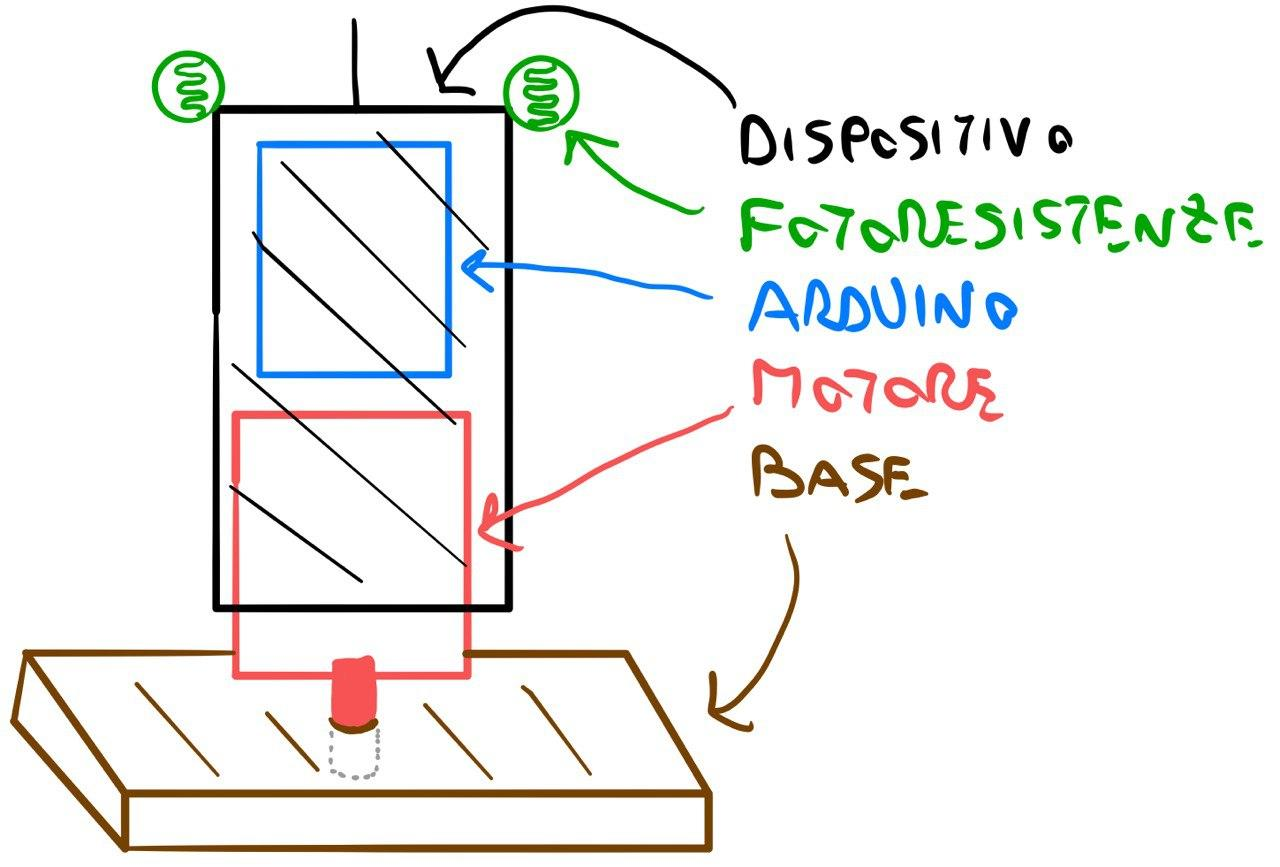
\includegraphics[width=0.5\textwidth]{figures/modello_solar_tracker}
    \caption{Struttura esemplificativa.}
\end{figure}

\subsection{Componenti}
Il dispositivo è stato realizzato con:
\begin{itemize}
    \item 1x Arduino NANO
    \item 1x 28BYJ-48 Stepper motor
    \item 1x ULN2003 driver board
    \item 2x Photoresistor GL5537
\end{itemize}
Tutti i componenti sono all'interno di una scatola tranne le fotoresistenze che si trovano nella parte superiore separate da un divisorio. La scelta di mettere tutti i componenti all'interno del case è stata fatta per permettere la completa rotazione, cosa che non si sarebbe potuto garantire altrimenti a causa dei cavi. (Il motore scelto non è il più adatto, ma essendo un prototipo a scopo didattico si è deciso di utilizzare quello già visto a lezione)

% \subsection{Considerazioni}
% Avendo utilizzato un solo motore è importante che la luce si sposti solo attorno alla normale al piano, al fine di vedere al meglio 

\subsection{funzionamento}
\begin{wrapfigure}{R}{0.3\textwidth}
    \centering
    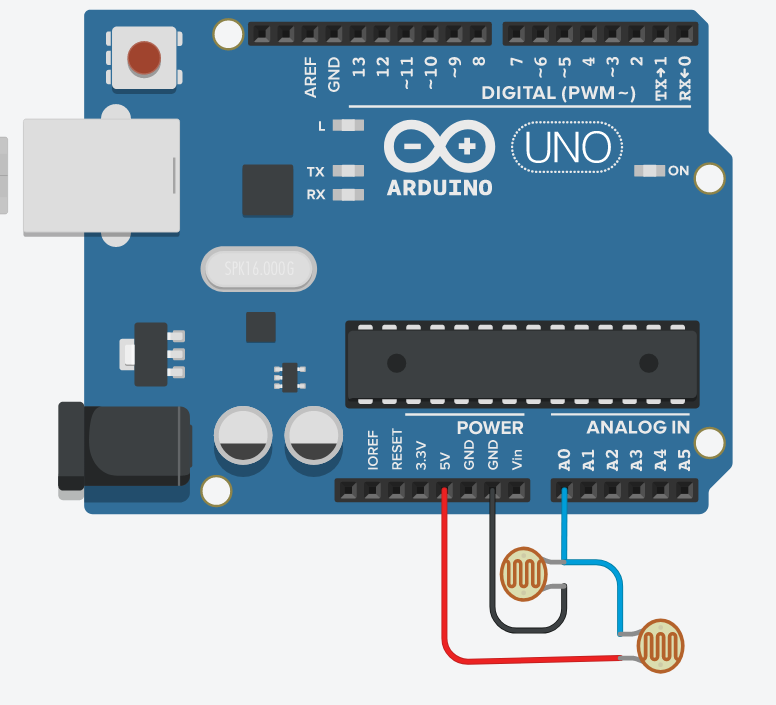
\includegraphics[width=0.25\textwidth]{figures/photoresistors}
    \caption{Collegamento fotoresistenze ad un Arduino UNO.}
\end{wrapfigure}
Il dispositivo ad un intervallo fissato (3 secondi) si riporta sempre alla posa che punta verso il punto con maggiore luce. Per farlo si legge il valore dell'ADC dell'analogInput dell'Arduino e lo si converte in tensione, dopodichè in base al risultato si farà girare il motore in senso orario o antiorario. Le due fotoresistenze sono disposte a formare un partitore di tensione, quindi:
\begin{itemize}
    \item se la tensione è 2.5V (cioè la metà della tensione leggibile) allora le due resistenze stanno facendo la stessa resistenza, ed essendo della stessa tipologia allora vuol dire che stanno ricevendo la stessa quantità di luce. Quindi in questa condizione non dobbiamo ruotare il dispositivo perchè siamo già nella posa voluta.
    \item se la tensione è maggiore di 2.5V allora la prima resistenza (ovvero quella che in figura è collegata direttamente coi 5V) sta facendo meno resistenza rispetto alla seconda e quindi è quella che sta ricevendo meno luce.
    \item se la tensione è minore di 2.5V allora la prima resistenza sta facendo più resistenza rispetto alla seconda e quindi è quella che sta ricevendo più luce.
\end{itemize}
Il controllo della luminosità viene fatto ad un intervallo fissato che varia in base al tipo di applicazione e serve per non far lavorare inutilmente, consumano energia, il dispositivo. Se per esempio si volesse far muovere il dispositivo in base alla luce solare allora questo intervallo andrebbe impostato a 30 minuti, invece per testare il dispositivo con una torcia elettrica bisognerebbe usare un intervallo di 3 secondi.
Dopo questo intervallo il dispositivo ad ogni ciclo deve leggere il valore di tensione data dalle fotoresistenze e dire al motore in che direzione andare fino alla ipotetica lettura del valore di 2.5V (cioè quando le due fotoresistenze ricevono la stessa quantità di luce). Essendo però difficile leggere esattamente il valore 2.5, il sistema risulterà instabile, continuando ad oscillare alla ricerca del punto di equilibrio. Per far fronte a questo problema, l'obiettivo non sarà più che l'input sia uguale a 2.5 ma minore di $2.5 - |epsilon|$.
Un primo approccio vede epsilon come numero fisso, ma questo valore dipende dalle condizione del sistema e rende impreciso il sistema. 
Un secondo approccio che supera queste limitazioni vede epsilon come numero variabile, che partendo da 0 cresce ogni volta che c'è una inversione di rotazione.


\section{Conclusioni}
Aggiungendo un altro motore è possibile estendere la ricerca della posa con più luce tenendo conto di tutte e 3 le dimensioni.
Grazie a questo miglioramento è possibile realizzare un dispositivo che permetta ad un pannello solare di essere posizionato sempre nella posizione che dia la maggior efficienza.


\bibliographystyle{ieeetr}
\bibliography{biblio}


\end{document}